\documentclass{article}

\usepackage{fancyhdr}
\usepackage{extramarks}
\usepackage{amsmath}
\usepackage{amsthm}
\usepackage{amsfonts}
\usepackage{tikz}
\usetikzlibrary{3d}
\usepackage[plain]{algorithm}
\usepackage{algpseudocode}
\usepackage{braket}
\usepackage{enumerate}
\usepackage{paralist}

%
% Basic Document Settings
%

\topmargin=-0.45in
\evensidemargin=0in
\oddsidemargin=0in
\textwidth=6.5in
\textheight=9.0in
\headsep=0.25in

\linespread{1.1}

\pagestyle{fancy}
\lhead{Habib University}
\chead{\hmwkClass, \hmwkTitle}
\rhead{\firstxmark}
\lfoot{\lastxmark}
\cfoot{\thepage}

\renewcommand\headrulewidth{0.4pt}
\renewcommand\footrulewidth{0.4pt}

\setlength\parindent{0pt}

%
% Create Problem Sections
%

\newcommand{\enterProblemHeader}[1]{
	\nobreak\extramarks{}{Problem \arabic{#1} continued on next page\ldots}\nobreak{}
	\nobreak\extramarks{Problem \arabic{#1} (continued)}{Problem \arabic{#1} continued on next page\ldots}\nobreak{}
}

\newcommand{\exitProblemHeader}[1]{
	\nobreak\extramarks{Problem \arabic{#1} (continued)}{Problem \arabic{#1} continued on next page\ldots}\nobreak{}
	\stepcounter{#1}
	\nobreak\extramarks{Problem \arabic{#1}}{}\nobreak{}
}

\setcounter{secnumdepth}{0}
\newcounter{partCounter}
\newcounter{homeworkProblemCounter}
\setcounter{homeworkProblemCounter}{1}
\nobreak\extramarks{Problem \arabic{homeworkProblemCounter}}{}\nobreak{}

%
% Homework Problem Environment
%
% This environment takes an optional argument. When given, it will adjust the
% problem counter. This is useful for when the problems given for your
% assignment aren't sequential. See the last 3 problems of this template for an
% example.
%
\newenvironment{homeworkProblem}[1][-1]{
	\ifnum#1>0
	\setcounter{homeworkProblemCounter}{#1}
	\fi
	\section{Problem \arabic{homeworkProblemCounter}}
	\setcounter{partCounter}{1}
	\enterProblemHeader{homeworkProblemCounter}
}{
	\exitProblemHeader{homeworkProblemCounter}
}

%
% Homework Details
%   - Title
%   - Due date
%   - Class
%   - Section/Time
%   - Instructor
%   - Author
%

\newcommand{\hmwkTitle}{Homework\ \#1}
\newcommand{\hmwkDueDate}{September 15, 2023, 11.59pm}
\newcommand{\hmwkClass}{CS 314/PHYS 300: Quantum Computing}
\newcommand{\hmwkClassInstructor}{Dr. Faisal Alvi}
\newcommand{\hmwkAuthorName}{\textbf{Student 1 Name, ID} \and \textbf{Student 2 Name, ID}}

%
% Title Page
%

\title{
	\vspace{2in}
	\textmd{\textbf{\hmwkClass:\\ \hmwkTitle}}\\
	\normalsize\vspace{0.1in}\small{\hmwkClassInstructor}\\
	\normalsize\vspace{0.1in}\small{Due\ on\ \hmwkDueDate}\\
	\vspace{3in}
}

\author{\hmwkAuthorName}
\date{}

\renewcommand{\part}[1]{\textbf{\large Part \Alph{partCounter}}\stepcounter{partCounter}\\}

%
% Various Helper Commands
%

% Useful for algorithms
\newcommand{\alg}[1]{\textsc{\bfseries \footnotesize #1}}

% For derivatives
\newcommand{\deriv}[1]{\frac{\mathrm{d}}{\mathrm{d}x} (#1)}

% For partial derivatives
\newcommand{\pderiv}[2]{\frac{\partial}{\partial #1} (#2)}

% Integral dx
\newcommand{\dx}{\mathrm{d}x}

% Alias for the Solution section header
\newcommand{\solution}{\textbf{\large Solution}}

% Probability commands: Expectation, Variance, Covariance, Bias
\newcommand{\E}{\mathrm{E}}
\newcommand{\Var}{\mathrm{Var}}
\newcommand{\Cov}{\mathrm{Cov}}
\newcommand{\Bias}{\mathrm{Bias}}

\begin{document}

\maketitle

\pagebreak

\begin{homeworkProblem}
	(10 points) Given a qubit $\ket{\psi} = \alpha \ket{0} + \beta \ket{1}$, and an operator denoted by a matrix $U$, prove that

	\begin{enumerate}[(a)]
		\item (5 points) if $U$ is unitary, then $U$ preserves the norm of the qubit after application, i.e., $|| \ket{\psi} || = ||\; U\ket{\psi} ||$.
		\item (5 points) alternately, if an operator $U$ is applied on a qubit that preserves the norm of the qubit, then it must be unitary.
	\end{enumerate}

	\textbf{Solution}
	Write solution here.
\end{homeworkProblem}

\begin{homeworkProblem}
	(10 points) Consider a Bloch Sphere representation of a qubit $\ket{\psi} = \cos(\theta/2)\ket{0} + e^{(i\phi)} \sin(\theta/2)\ket{1}$ as shown here.

	\begin{figure} [H]
		\centering
		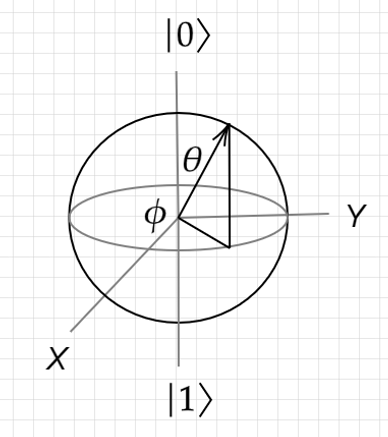
\includegraphics[scale = 0.7]{Bloch-Sphere.png}
		\caption{Bloch sphere representation of an arbitrary qubit state $\ket{\psi} = \cos(\theta/2)\ket{0} + e^{(i\phi)} \sin(\theta/2)\ket{1}$}
	\end{figure}
	On the Bloch Sphere, plot the following qubits (show a plot similar to a diagram above):
	\begin{enumerate}[(a)]
		\item (2 points) \[\frac{\sqrt{3}}{2}|0\rangle + \frac{1}{2}|1\rangle\]
		\item (3 points) \[ \frac{1+i}{2}|0\rangle + \frac{1-i}{2}|1\rangle\]
	\end{enumerate}
	Next, consider the following operations:
	\[
		(i) \;\;	R(\theta_1) = \begin{bmatrix}
			\cos(\theta_1) & -\sin(\theta_1) \\
			\sin(\theta_1) & \cos(\theta_1)
		\end{bmatrix},
		(ii) \;\;	S(\phi_2) = \begin{bmatrix}
			1 & 0           \\
			0 & e^{i\phi_2}
		\end{bmatrix}\]
	Given an arbitrary qubit on the $X$-$Z$ plane (i.e.) its amplitudes have no imaginary component, \\

	(a) (2 points) what is the effect of applying $R(\theta_1)$ to it? In particular state the effect when $\theta_1 = \pi/2$?\\

	(b) (3 points) what is the effect of applying $S(\phi_2)$ to it? In particular state the effect when $\phi_2 = \pi/2$?\\

\end{homeworkProblem}

\begin{homeworkProblem}
	(10 points) So far we have studied qubits defined using two basis states: $\ket{0}$ and $\ket{1}$. We have also seen two related states: the $\ket{+}$ state and the $\ket{-}$ state. Answer the following questions with reasons:

	\begin{enumerate}[(a)]
		\item(2 points) Do the $\ket{+}$ state and the $\ket{-}$ state form a pair of orthonormal states?
		\item (2 points) Can the $\ket{+}$ state and the $\ket{-}$ state be used as the basis states?
		\item If the answer to the both (a) and (b) is Yes, express the following qubits as a linear combination of the $\ket{+}$ state and the $\ket{-}$ state:

		      (i) (2 points) $\ket{0}$,

		      (ii) (2 points) $\ket{1}$,

		      (iii) (2 points) an arbitrary qubit: $\ket{\psi} = \alpha \ket{0} + \beta \ket{1}$.

	\end{enumerate}

\end{homeworkProblem}



\begin{homeworkProblem}
	The Pauli Matrices are given by:

	\begin{align*}
		X = \sigma_x & = \begin{pmatrix}
			                 0 & 1 \\
			                 1 & 0
		                 \end{pmatrix} \\
		Y = \sigma_y & = \begin{pmatrix}
			                 0 & -i \\
			                 i & 0
		                 \end{pmatrix} \\
		Z = \sigma_z & = \begin{pmatrix}
			                 1 & 0  \\
			                 0 & -1
		                 \end{pmatrix}
	\end{align*}


	Show that the following relations hold:
	\vspace{2pt}
	\begin{compactenum}[(a)]
		\item (3 points) $HX$ = $ZH$, \\
		\item (3 points) $HY$ = $-YH$, \\
		\item (3 points) $HZ$ = $XH$. \\
	\end{compactenum}
	where $H$ is the Hadamard operation.
	\vspace{2pt}

	(1 point) Using these properties, show that $HXHYHZ = -ZYXH$

\end{homeworkProblem}

\begin{homeworkProblem}
	We have seen earlier that if we are given one of the two quantum states $\ket{+}$ and $\ket{-}$ such that it is not known whether it is a $\ket{+}$ and $\ket{-}$, we can distinguish between them \textit{perfectly} by applying a Hadamard operation followed by a measurement. \\


	Suppose we are randomly sent one of the following two states: \[ (a) \;\;
		\frac{1}{2}\ket{0} + \frac{\sqrt{3}}{2}\ket{1}, (b) \;\; \frac{\sqrt{3}}{2}\ket{0} - \frac{1}{2}\ket{1},
	\]

	Devise a procedure to find out which one of the two states has been sent that performs better than a random choice. More specifically, given one of the two qubits, by performing your operation(s) followed by a measurement, the probability of finding out which one of the states is greater than random guessing i.e. greater than 1/2.

\end{homeworkProblem}

\end{document}